\documentclass[article,type=msc,colorback,accentcolor=tud7b]{tudthesis}

%TODO: Markus Zopf

\usepackage[english]{babel}
\usepackage{amsmath}
\usepackage{array}
\usepackage{enumitem}
\usepackage{listings}
\usepackage{floatrow}
\usepackage{multirow}
\usepackage{subfig}
% Table float box with bottom caption, box width adjusted to content
\newfloatcommand{capbtabbox}{table}[][\FBwidth]
\restylefloat{table}
\newcolumntype{C}[1]{>{\centering\let\newline\\\arraybackslash\hspace{0pt}}m{#1}}

\usepackage[
    backend=biber, % biber ist das Standard-Backend für Biblatex. Für die Abwärtskompatibilität kann hier auch bibtex oder bibtex8 gewählt werden (siehe biblatex-Dokumentation)
    style=alphabetic, %numeric, authortitle, alphabetic etc.
    autocite=plain, % Stil, der mit \autocite verwendet wird
    sorting=nty, % Sortierung: nty = name title year, nyt = name year title u.a.
    sortcase=false,
    url=false,
    hyperref=auto,
]{biblatex}

\addbibresource{bibliography.bib}

\newcommand{\getmydate}{%
  \ifcase\month%
    \or Januar\or Februar\or M\"arz%
    \or April\or Mai\or Juni\or Juli%
    \or August\or September\or Oktober%
    \or November\or Dezember%
  \fi\ \number\year%
}

\begin{document}
  \thesistitle{Sentiment classification of chess annotations}{}
  \author{Florian Beck}
  \referee{Prof. Dr. Johannes Fürnkranz}{}
  \department{Fachbereich Informatik}
  \group{Knowledge Engineering Group}
  \dateofexam{\today}{\today}
  %\tuprints{12345}{1234}
  \makethesistitle
  \affidavit{Florian Beck}
  
  \input{abstract}
  %TODO: auch in deutsch
  \clearpage
  
  \setcounter{tocdepth}{3}
  \tableofcontents
  \setcounter{page}{3}
  \clearpage
  
  \listoffigures
  \listoftables
  \clearpage
  
  \section{Introduction}

  \subsection{Motivation}

  \subsection{Problem Description}

  \subsection{Goal of the Thesis}
    - is it possible to "convert" a chess annotation comment to the appropiate symbol by using a classifier

  \subsection{Structure of the Thesis}
  \clearpage
  
  \section{Fundamentals}
  
  \subsection{Text Mining}
  
  \subsection{Sentiment Analysis}

  \subsection{Word Embeddings}
  \label{subsec:word_embeddings}
    
    \begin{figure}[H]
      \centering
      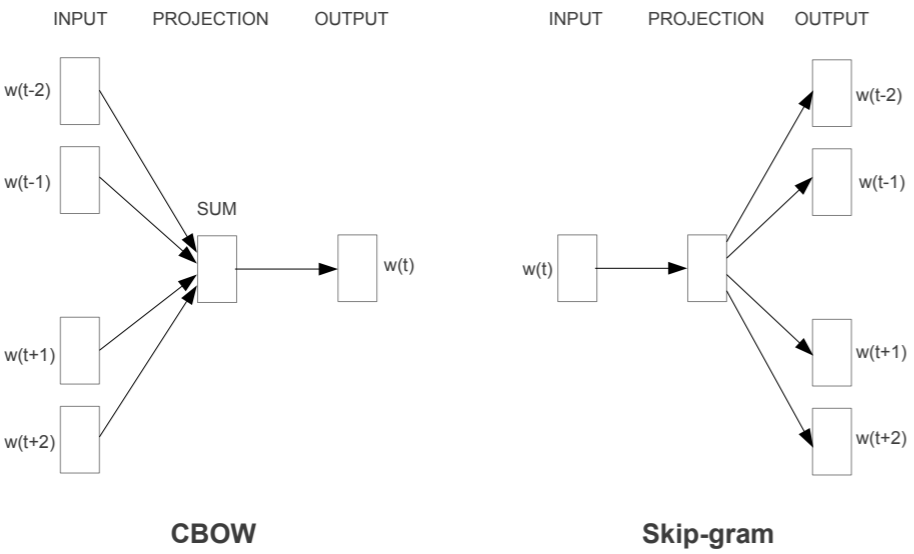
\includegraphics{images/word_embeddings}
      \caption[CBOW and Skip-gram model]{CBOW and Skip-gram model \autocite{Mikolov2013}}
      \label{fig:word_embeddings}
    \end{figure}
    
  \clearpage
  
  \subsection{Multiclass Classification}
  \label{subsec:multiclass_classification}  
    Multiclass classification is a problem in the field of supervised learning. The task is the prediction of one class out of a finite set of three or more possible classes for each instance. As can be seen in figure~\ref{fig:problem_hierarchy_supervised_learning}, it can be distinguished from other problems in supervised learning. First, as the name implies, it is a classification problem because the range of values is finite rather than continuous, as is the case with a regression problem. Furthermore, each instance should be associated with exactly one class, which distinguishes it from the similar sounding multi-label classification, since each instance can be associated with any number of classes (= labels). Finally, the model to be learned has to choose from a set of $k$ classes with $k>2$, i.e. $\{1,2,\dots,k\}$. This makes the problem slightly more difficult than binary classification with $k=2$. Ordinal classification is a specialization of multiclass classification and will be discussed in detail in subsection~\ref{subsec:ordinal_classification}.
    
    \begin{figure}[H]
      \centering
      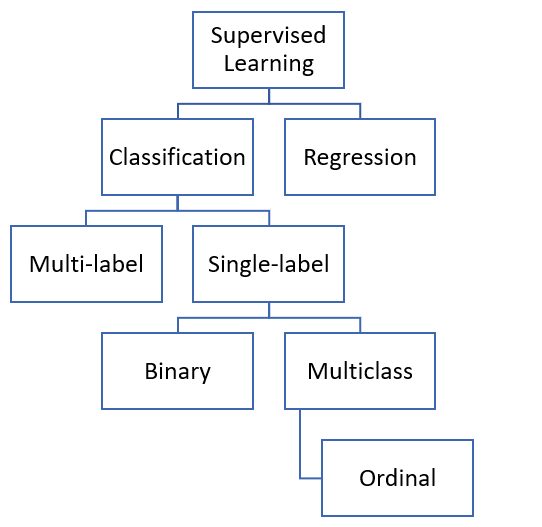
\includegraphics{images/problem_hierarchy_supervised_learning}
      \caption{Problem hierarchy of supervised learning}
      \label{fig:problem_hierarchy_supervised_learning}
    \end{figure}
    
    Most algorithms applied to classification problems are explained by their application to binary classification problems, which cover a large part of the real-world use cases. However, these approaches cannot be adopted to multiclass problems without further ado. \citeauthor{Aly2005} describes with the decomposition into binary classification, hierarchical classification and the extension of algorithms the three groups of approaches to cope with the difficulties of multiclass classification \autocite{Aly2005}:
    \begin{itemize}
      \item Decomposition into Binary Classification

        A frequently chosen approach is the transformation of the multiclass classification problem into several binary classification subproblems, for which there are three different possibilities. In any case the results of subproblems have to be joined to be able to make a final prediction which is similar to ensemble learning. \\\\
        The first option called one-against-all splits the multiclass classification problem into $k$ binary classification subproblems. The classifier $f_{i}$ treats the instances of class $i$ as positive and instances of the $k-1$ other classes as negative. An example of one-against-all using an SVM-classifier is shown in figure~\ref{fig:one_against_all_or_one} on the left. For an unseen instance $x$ the class $k$ with the highest confidence score will be predicted:
        \[y(x)=\underset{i\in\{1 \dots k\}}{\operatorname{argmax}} f_{i}(x)\]
        However, there is no guarantee that the real-valued quantities $f_{i}(x)$ for different classifiers will have appropriate scales. Furthermore, especially for a high $k$ the ratio between positive and negative instances is low, which complicates the creation of a model. This problem can be addressed by giving greater weight to the positive instances \autocite[Subsection~7.1.3]{Bishop2006}.

        \begin{figure}[H]
          \centering
          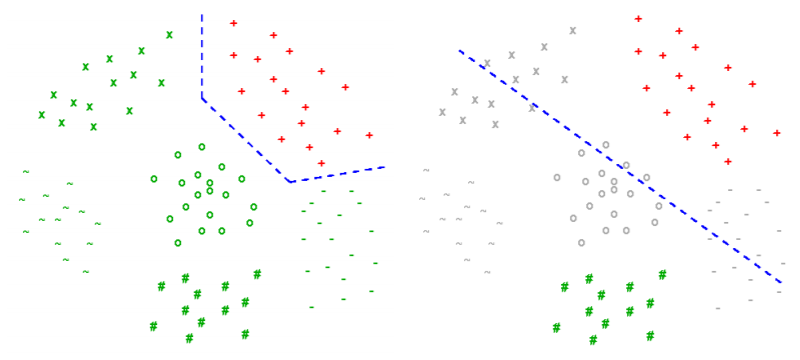
\includegraphics{images/one_against_all_or_one}
          \caption[One-against-all vs. one-against-one approach]{One-against-all (left) vs. one-against-one approach (right)\protect\footnotemark}
          \label{fig:one_against_all_or_one}
        \end{figure}
    
        \footnotetext{J. Fürnkranz, Machine Learning and Data Mining | Learning Rule Sets, V3.0, p.45\&47}

        The second option called one-against-one splits the multiclass classification problem into even more binary classification subproblems, in fact $\frac{k(k-1)}{2}$. This number results from the fact that now in each subproblem two classes are pairwise distinguished from each other. Since in the binary classifier between the classes $i$ and $j$ all instances of the classes except $i$ and $j$ can be discarded (see figure~\ref{fig:one_against_all_or_one} on the right), there are smaller subproblems than in one-against-all, which usually also create simpler models. However, the number of subproblems is $\frac{k}{2}$-times as high, which usually results in significantly more training time \autocite[Subsection~7.1.3]{Bishop2006}. \\
        The final decision is made by voting. All pairwise comparisons are summed up and the winner with the most partial victories is the output class. However, using the binary outputs of the subproblems, i.e. only the preferred class, often leads to several winners. There are different ways to handle these ambiguities. The first idea is weighting the subproblems differently, for example by modifying the output from $1$ to the accuracy and from $0$ to $1-$accuracy. Another idea called pairwise coupling can be used which includes probabilities for every subproblem in the calculation. \citeauthor{Wu2004} present a few pairwise coupling techniques that are more stable than using the simple voting approach \autocite{Wu2004}. \\\\

        The third option is the usage of error-correcting output codes. Each class is assigned to a unique binary string of length $n$; we will refer to these strings as “codewords”. During training for an example from class $i$, the desired outputs of these $n$ binary functions are specified by the codeword for class $i$. With artificial neural networks, these $n$ functions can be implemented by the $n$ output units of a single network \autocite[Section~1]{Dietterich1994}. Though, it is also possible to train all $n$ binary classifiers individually with an arbitrary algorithm. A test instance is assigned to the class that is closest to the code determined by the $n$ functions. \\
        Now the question arises, how the codewords respectively the binary functions are chosen most effectively. Out of all $2^{k}$ binary combinations for a $k$-class problem, after removing $2^{k-1}$ complements (e.g. all starting with $1$) and the uniform classifier there are $2^{k-1}-1$ possible classifiers, from which to be selected. A good error-correcting output code for a $k$-class problem should satisfy two properties \autocite[Subsection~2.3]{Dietterich1994}:
        \begin{itemize}
          \item Row Separation

            If in a code converting an arbitrary codeword into another arbitrary codeword needs $d$ changes of bits, the code has a so-called Hamming distance of $d$. The higher the Hamming distance, the better the row separation. A code with Hamming distance $d$ can detect up to $d-1$ and correct up to $\left\lfloor\frac{d-1}{2}\right\rfloor$ bits.
          \item Column Separation

            Each bit-position function $f_{i}$ should be uncorrelated with the functions to be learned for the other bit positions $f_{j}$; $j\neq i$. If two columns $i$ and $j$ (or the complement of $j$) are similar or identical, then when a deterministic learning algorithm such as the decision tree classifier C4.5 is applied to learn $f_{i}$ and $f_{j}$, it will make similar (correlated) mistakes.
        \end{itemize}
        The classifier sets in the one-against-all and one-against-one approaches are feasible solutions. The one-against-all approach guarantees Hamming distances of $2$ for both row and column separation, the one-against-one approach even $2\times(k-2)$ for the row and $4$ (if $k>7$) for the column separation. The optimal row distance is achieved by the union of all $2^{k-1}-1$ binary combinations and called exhaustive code. Until $k=5$ the exhaustive code is just the union of all classifiers of the one-against-all and one-against-one approaches (or their inversions, see table~\ref{tab:exhaustive_ecoc}), but for $k>6$ the number of additional classifiers increases quickly, wherefore instead of an exhaustive code also a suitable subset of those classifiers can be sufficient and improve the column separation.
  
        \begin{table}[H]
          \centering
          \setlength\tabcolsep{1.5pt}
          \subfloat[One-against-all]{
          \begin{tabular}{ |C{1.5cm}|C{0.5cm}|C{0.5cm}|C{0.5cm}|C{0.5cm}|C{0.5cm}| } 
            \hline
            class & $f_{1}$ & $f_{2}$ & $f_{3}$ & $f_{4}$ & $f_{5}$ \\ \hline
            1 & 1 & 0 & 0 & 0 & 0 \\ \hline
            2 & 0 & 1 & 0 & 0 & 0 \\ \hline
            3 & 0 & 0 & 1 & 0 & 0 \\ \hline
            4 & 0 & 0 & 0 & 1 & 0 \\ \hline
            5 & 0 & 0 & 0 & 0 & 1 \\ \hline
          \end{tabular}
          }
          \quad
          \subfloat[One-against-one]{
          \begin{tabular}{ |C{1.5cm}|C{0.5cm}|C{0.5cm}|C{0.5cm}|C{0.5cm}|C{0.5cm}|C{0.5cm}|C{0.5cm}|C{0.5cm}|C{0.5cm}|C{0.5cm}| } 
            \hline
            class & $f_{1}$ & $f_{2}$ & $f_{3}$ & $f_{4}$ & $f_{5}$ & $f_{6}$ & $f_{7}$ & $f_{8}$ & $f_{9}$ & $f_{10}$ \\ \hline
            1 & 1 & 1 & 1 & 1 & 0 & 0 & 0 & 0 & 0 & 0 \\ \hline
            2 & 1 & 0 & 0 & 0 & 1 & 1 & 1 & 0 & 0 & 0 \\ \hline
            3 & 0 & 1 & 0 & 0 & 1 & 0 & 0 & 1 & 1 & 0 \\ \hline
            4 & 0 & 0 & 1 & 0 & 0 & 1 & 0 & 1 & 0 & 1 \\ \hline
            5 & 0 & 0 & 0 & 1 & 0 & 0 & 1 & 0 & 1 & 1 \\ \hline
          \end{tabular}
          }
      
          \subfloat[Exhaustive error-correcting output code]{
          \begin{tabular}{ |C{1.5cm}|C{0.5cm}|C{0.5cm}|C{0.5cm}|C{0.5cm}|C{0.5cm}|C{0.5cm}|C{0.5cm}|C{0.5cm}|C{0.5cm}|C{0.5cm}|C{0.5cm}|C{0.5cm}|C{0.5cm}|C{0.5cm}|C{0.5cm}| } 
            \hline
            class & $f_{1}$ & $f_{2}$ & $f_{3}$ & $f_{4}$ & $f_{5}$ & $f_{6}$ & $f_{7}$ & $f_{8}$ & $f_{9}$ & $f_{10}$ & $f_{11}$ & $f_{12}$ & $f_{13}$ & $f_{14}$ & $f_{15}$ \\ \hline
            1 & 0 & 0 & 0 & 0 & 0 & 0 & 0 & 0 & 0 & 0 & 0 & 0 & 0 & 0 & 0 \\ \hline
            2 & 0 & 0 & 0 & 0 & 0 & 0 & 0 & 1 & 1 & 1 & 1 & 1 & 1 & 1 & 1 \\ \hline
            3 & 0 & 0 & 0 & 1 & 1 & 1 & 1 & 0 & 0 & 0 & 0 & 1 & 1 & 1 & 1 \\ \hline
            4 & 0 & 1 & 1 & 0 & 0 & 1 & 1 & 0 & 0 & 1 & 1 & 0 & 0 & 1 & 1 \\ \hline
            5 & 1 & 0 & 1 & 0 & 1 & 0 & 1 & 0 & 1 & 0 & 1 & 0 & 1 & 0 & 1 \\ \hline
          \end{tabular}
          }
          \caption[Output codes for a multiclass classification problem]{Different output codes for a multiclass classification problem with five classes}
          \label{tab:exhaustive_ecoc}
        \end{table}

        The exhaustive error-correcting code for $k=5$ is shown in table~\ref{tab:exhaustive_ecoc}. The hamming-distance of the code is $d=8$. Therefore, the code can detect up to $d-1=7$ and correct up to $\left\lfloor\frac{d-1}{2}\right\rfloor=3$ bits. Error-correcting output codes are a robust alternative to one-against-all and one-against-one approaches which outperforms them in most cases but also entail the disadvantages of a more complex training and model \autocite[Section~4]{Dietterich1994}.
      \item Hierarchical Classification

        Hierarchical classification, also known as nested dichotomies, is strictly speaking also a type of decomposition of a multiclass classification problem into binary classification problems. However, in this approach the output of the classifiers is not always used for the prediction but as the input for the next classifier. In this way, a hierarchy of classifiers and their subproblems is created. The first classifier is trained on the whole input space; the total set of all classes is suitably divided into two subsets between which the classifier distinguishes. This procedure is then continued recursively with the two subsets until all subsets only contain instances of a single class. This procedure creates a tree structure whose leaves are the set of instances of a class. As a result, this tree contains $k$ leaves and $k-1$ inner nodes representing the binary classifiers \autocite{Dong2005}. Two possibly outcomes of a multiclass classification problem with $5$ classes are shown in figure~\ref{fig:nested_dichotomies}.

        \begin{figure}[H]
          \centering
          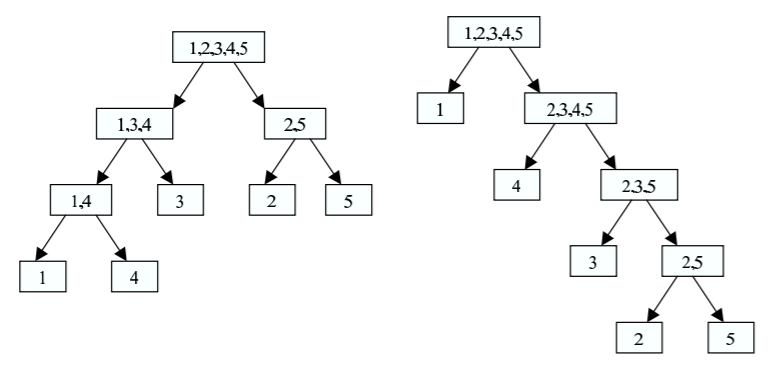
\includegraphics{images/nested_dichotomies}
          \caption[Two nested dichotomies]{Two nested dichotomies for a multiclass problem with five classes \autocite{Dong2005}\protect\footnotemark}
          \label{fig:nested_dichotomies}
        \end{figure}

        The probability of a class can be calculated by multiplying all probability estimates of the classifier along the path from the root to the class. This value differs for disparate nested dichotomies, wherefore usually various trees are computed and their probabilities are averaged. Though, for high $k$ there are too many different possibilities to build a nested dichotomy. Balanced nested dichotomies prove to be particularly suitable, since they require the shortest running time without affecting the accuracy negatively \autocite{Dong2005}. \citeauthor{Dong2005} developed methods to balance the nested dichotomies either by class or by data amount.
      \item Extension of Algorithms

        The third idea is the inversion of the first two approaches. Instead of modifying the problem and using the same classifier as for the binary classification, we now modify the classifier such that we can leave the classifier unchanged. Typical algorithms in machine learning are decision trees, pattern- or rule-based classifiers, probabilistic classifiers, SVM classifiers, neural network classifiers and proximity-based classifiers. A short description for every algorithm can be found in subsection~\ref{subsec:analysis}. Decision trees, pattern- or rule-based classifiers, probabilistic classifiers as Naïve Bayes and proximity-based classifiers as $k$-nearest-neighbor can be easily adapted to multiclass problems. For the other two algorithms some preliminary considerations are necessary. \\\\
        SVM classifiers use hyperplanes of dimension $D-1$ described by linear functions to separate the whole input space of dimension $D$ into two subspaces which ideally only contain a single class. Obviously, a single hyperplane is not sufficient for separating more than two classes. Approaches like one-against-all and one-against-one lead to ambiguous subspaces where either more than one class or no class is assigned to. We can avoid these difficulties by considering a single $k$-class discriminant comprising $k$ linear functions (with parameters $\mathbf{w}_{i}$ and $w_{i 0}$) of the form
        \[y_{i}(\mathbf{x})=\mathbf{w}_{i}^{\mathrm{T}} \mathbf{x}+w_{i 0}\]
        and then assigning a point $\mathbf{x}$ to class $i$ if $y_{i}(\mathbf{x})>y_{j}(\mathbf{x})$ for all $j\neq i$. The decision boundary between class $i$ and class $j$ is therefore given by $y_{i}(\mathbf{x})=y_{j}(\mathbf{x})$ and hence corresponds to a $(D-1)$-dimensional hyperplane defined by
        \[\left(\mathbf{w}_{i}-\mathbf{w}_{j}\right)^{\mathrm{T}} \mathbf{x}+\left(w_{i 0}-w_{j 0}\right)=0.\]
        The decision regions of such a discriminant are always singly connected and convex \autocite[Subsection~4.1.2]{Bishop2006}. \\\\
        A neural network classifier has in general $n$ neurons in the output layer, each of them with a binary output. For binary classification problems, a single neuron in the output layer, i.e. $n=1$, is sufficient since it only needs to distinguish between two classes, represented by the two outputs $0$ and $1$. For multiclass classification problems, $n=1$ is not sufficient. The straightforward solution would be to define $n=k$ neurons in the output layer, one for each of the $k$ classes. But already $\left\lfloor\log_{2}k\right\rfloor$ output neurons are enough if the classes are encoded as the first $k$ numbers in binary representation. By using error-correcting output codes containing more than $\left\lfloor\log_{2}k\right\rfloor$ output neurons, the binary code can also be made more resistant to errors \autocite[Subsection~2.1]{Aly2005}.
    \end{itemize}
    As mentioned in the beginning of this subsection, ordinal classification problems are a subgroup of multiclass classification problems. The following subsection describes the special properties of this type of problems and other approaches that are even better adapted to these properties than those presented here.

  \subsection{Ordinal Classification}
  \label{subsec:ordinal_classification}
    Ordinal classification problems are a specialization of multiclass classification problems. They refer to an important category of real-world problems, in which the classes exhibit a natural order. Thus, the class attribute is not nominal, but ordinal. However, the possibility of calculating the difference (essential for an interval class attribute) or even the quotient (essential for a ratio class attribute) is usually not given \autocite[Section~1]{Frank2001}. Ordinal classification may be viewed as a bridging problem between the two standard machine-learning tasks of classification and regression, because the set of classes has the property of a finite range given in classification problems as well as the property of a natural order given in regression problems \autocite[Section~1]{Kotsiantis2004}. \\\\
    As a specialization of a multiclass classification problem, ordinal classification problems can be approached with the same strategies as described above in subsection~\ref{subsec:multiclass_classification}. However, the additional information of the linear order of the classes is ignored. Two strategies tailored to ordinal classification problems taking this information into account are ordinal regression and an adapted transformation to binary classification problems.
    \begin{itemize}
      \item Ordinal Regression

        In regression tasks, the output is a numeric value in a continuous range. The idea of ordinal regression is to treat the ordinal output as a numeric value. In this way the same approaches as for regression tasks can be used only with the extension that the predicted values still have to be mapped to the fixed classes. Nevertheless, most regression methods require some metric assumptions like building differences or ratios within the ordinal scale \autocite[Section~1]{Ruan2014}. Hence the result of the model depends on the choice of numeric values and their distances from each other. This leads to problems in many real-world applications, for example in the quantification of ordinal scales in opinion surveys. \\\\
        Ordinal logistic models avoid this issue by only considering the ranking order of the classes \autocite[Chapter~13]{Harrell2015}. The most commonly used ordinal logistic model is the proportional odds model. It uses the logarithms of odds that the predicted class $y$ is one of the first $i$ classes together with a linear function, whereby the probability after forming is given by
        \[\operatorname{P}(y\leq i|\mathbf{x})=\frac{1}{1+\exp\left[-\left(\mathbf{w}^{\mathrm{T}}\mathbf{x}+w_{i 0}\right)\right]}\]
        where $\mathbf{x}$ is the test instance and $\mathbf{w}$ and $w_{i 0}$ the parameters of the linear function. There are many possible extensions to this ordinal model, among others replacing the cumulative probabilities with conditional probabilities or using a hazards model \autocite[Chapter~13]{Harrell2015}. 
      \item Transformation to Binary Classification Problems
      
        A simpler approach using a transformation to binary classification problems is presented by \citeauthor{Frank2001}. In contrast to the binary classification approaches in multiclass classification it takes advantage of the order of the classes. The ordinal class attribute with ordered values $v_{1}<v_{2}<\dots< v_{k}$ is converted into $k-1$ binary attributes. The $i$-th binary attribute represents the test if the class attribute exceeds the value of the $i$-th class: $x>v_{i}$. This construction of binary attributes requires exactly two classifiers and their probabilities to determine whether a test instance $x$ belongs to a class $i$:
        \[\operatorname{P}\left(v_{i}\right)=\operatorname{P}\left(x>v_{i-1}\right)-\operatorname{P}\left(x>v_{i}\right)\]
        For the highest class, the first probability is $1$ and for the lowest, the second is $0$, which further simplifies the calculation. Finally, the class with the highest probability is predicted. \citeauthor{Frank2001} showed that for ordinal classification problems this approach outperforms the “naïve” one-against-all algorithm, which treats the class values as an unordered set \autocite{Frank2001}.
    \end{itemize}
  
  \subsection{Cost-sensitive Learning}
  \label{subsec:cost_sensitive_learning}
    In many classification problems the goal is the optimization of some performance measurement, most often the accuracy. However, the best solution in respect to the accuracy does not have to be the one with minimized costs, which is also often a goal to be achieved. Costs can not only arise from misclassifications, but also from additional tests or time for the creation of a better model. \citeauthor{Turney2002} divides the reasons for costs that a machine learning problem can entail into nine groups \autocite{Turney2002}:
    \begin{itemize}[noitemsep]
      \item misclassification errors
      \item tests
      \item teacher
      \item intervention
      \item unwanted achievements
      \item computation
      \item cases
      \item human-computer interaction
      \item instability
    \end{itemize}
    In each of the nine groups, we can distinguish between constant and conditional costs. In the case of test costs, we speak of constant costs if a certain test has a fixed cost value for its execution. Note that different test may have different costs if they still remain constant for all instances in all circumstances. On the contrary, conditional test costs depend on a criterion. For a medical test this criterion might be the test result, the age of a patient or the result of prior tests. In the remaining subsection, of all cost types only the misclassification costs are discussed and therefore abbreviated to costs. \\\\
    The standard approach to evaluate the performance of a classifier is the calculation of the accuracy, i.e. the number of correct classified instances in relation to the total number of instances. The error costs result directly from the number of misclassified instances, which only has to be multiplied by a constant cost factor. Thus, \citeauthor{Turney2002} calls this value constant misclassification error cost. However, there are various problems in machine learning where such a simplification would lead to a miscalculation of the total costs because the conditional error costs are ignored. \\\\
    In many cases, the equal treatment of all error types is the cause of the incorrect cost estimate. For this we first consider the binary classification with only two classes and therefore only two possible error types. A false positive (FP) occurs when the outcome is incorrectly predicted as yes (or positive) when it is actually no (or negative). The reverse case is called false negative (FN). False positives and false negatives have rarely equal costs in real-world applications. In spam-classification, a no-spam e-mail classified as spam is worse than a spam e-mail which have not been detected correctly. An accepted customer which is not capable of paying back a loan has bigger costs than a customer wrongly classified as insolvent. A sick patient who is classified as healthy is more problematic than a healthy patient who is classified as sick. In order to map this, a cost value is determined for each of the two errors FP and FN or the cost ratio is determined. \\\\
    If we transfer the cost calculation to the multiclass classification, there are more error types and therefore more cost factors to be defined: Each instance of class $i$, misclassified as class $j$ will be multiplied with the correspondent cost factor $c_{ij}$. For a multiclass classification problem with $n$ classes we get a $n\times n$ cost matrix similar to the confusion matrix, which has $n(n-1)$ possibly different cost factors and whose main diagonal contains zeros. \\\\
    A special case arises for classification problems with ordinal classes. The value of $c_{ij}$ should reflect the extent of the difference between $i$ and $j$. Thus, it is common to assume that $c_{ij}=0$ when $i=j$. In addition, the cost $c_{ij}$ is assumed to be larger when $i$ is further away from $j$. Two common functions satisfy the requirements and have been widely used in practice \autocite[Section~3.1]{Ruan2014}:
    \begin{itemize}
      \item \makebox[4cm][l]{Absolute cost vectors} $c_{ij}=\left|i-j\right|$
      \item \makebox[4cm][l]{Squared cost vectors} $c_{ij}=\left(i-j\right)^{2}$
    \end{itemize}
    Note that the squared cost charges more than the absolute cost when $i$ is further away from $j$. The cost matrix of a multiclass classification problem with $n$ classes using absolute cost vectors looks like this \autocite[Section~3]{Kotsiantis2004}:
    \[\left[ \begin{array}{ccccc}
    {0} & {1} & {2} & {\dots} & {n-1} \\
    {1} & {0} & {1} & {\dots} & {n-2} \\
    {\dots} & {\dots} & {\dots} & {\dots} & {\dots} \\
    {n-2} & {\dots} & {1} & {0} & {1} \\
    {n-1} & {\dots} & {2} & {1} & {0}
    \end{array}\right]\]
    By squaring each element of the matrix, one obtains the matrix of squared cost vectors. In both cases it is a symmetrical matrix, i.e. $c_{ij}=c_{ji}\forall i,j\in\{1, \dots, m\}$. In some cases, it may be useful to weight the over- and underestimation of classes differently. If the overestimation of a class is to be penalized more severely than the underestimation, all elements to the right of the main diagonal are multiplied by a constant value $\lambda>1,\lambda\in\mathbb{R}$. In a comparable way all values of the matrix can be adjusted as required to the problem which has to be solved. \\\\
    Given such a cost matrix, you can calculate the cost of a particular learned model on a given test set just by summing the relevant elements of the cost matrix for the model’s prediction for each test instance. Here, the costs are ignored when making predictions, but taken into account when evaluating them \autocite[Chapter~5.7]{Witten2005}. In this way the classifier obviously does not have to deliver the cost-optimal result. However, there are different possibilities to include costs in advance \autocite[Chapter~2.3]{Qin2010}:
    \begin{itemize}
      \item Change of the class distribution of the training data
        
        This approach incorporates the misclassification cost into the data pre-processing step by re-sampling or re-weighting the training data in proportion of their misclassification cost.
      \item Modification of the learning algorithm
        
        This approach modifies the error-based classifiers directly to handle misclassification cost, but each classifier needs to be modified separately.
      \item Boosting approach
        
        This approach generates a set of different weak classifiers in sequential trial and then constructs a composite classifier by voting them. The advantage of this approach is that it is applicable to any kind of error-based classifiers.
      \item Conditional probability estimates / Direct cost-sensitive learning
        
        This approach incorporates the misclassification cost into the data post-processing step by using the probability estimation generated by error-based classifiers and the cost function to directly compute the optimal class for each test example. This approach is easy to implement, but needs good calibration methods to generate accurate probability estimation.
    \end{itemize}
Note that the use of the costs as in one of the approaches presented here does not preclude a subsequent evaluation of the costs. In this way it can be checked whether a classifier who incorporates the costs into the learning process is actually superior to a classifier without knowledge of the costs.

  \clearpage
  
  \section{Concept}
  
    This chapter describes how to solve a general problem of extracting knowledge out of natural language sources and defines which steps have to be considered. Therefore, in the following the focus is set on universal approaches to accomplish such a task. Specific ideas and solutions adjusted to the sentiment classification task for chess annotations will be dealt with in section~\ref{sec:experimental_setup}. \\\\
    The solution of a text mining problem comprises several steps from definition to evaluation. Figure~\ref{fig:text_mining_pipeline} shows a possible process model based on approaches of \citeauthor{Schieber2014} \autocite{Schieber2014} and \citeauthor{Kwartler2017} \autocite{Kwartler2017}. The model consists of six steps, which are now presented one after the other.
    
    \begin{figure}[H]
      \centering
      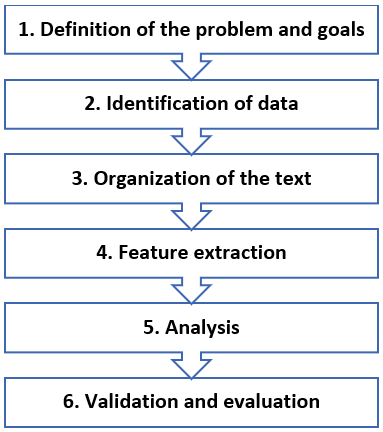
\includegraphics{images/text_mining_pipeline}
      \caption{Processing pipeline of text mining}
      \label{fig:text_mining_pipeline}
    \end{figure}
  
  \subsection{Definition of the Problem and Goals}
  \label{subsec:definition_of_the_problem_and_goals}
    In the first step we have to define the problem we want to solve. According to \citeauthor{Mitchell1997} a learning problem generally reads as follows: Improve over task $T$, with respect to performance measure $P$, based on experience $E$. The goal is therefore to generalize the experience in a way that allows to improve your performance on the task \autocite[Chapter~1]{Mitchell1997}.
    \begin{itemize}
      \item Task $T$
      
        The task can be formulated by a simple verbal description, e.g. “play the game Connect Four” or “sort the e-mail into the categories spam and no-spam”. A more formally approach requires the exact definition of the input and the output of the task. \\
        The input could be a set of attribute-value pairs, e.g. in relational data, where each input would have the same set of attributes. But since there is no restriction to the input data to be homogeneous the input can be plain text as well. A possible input of natural language could be represented by a whole book, by a (web) page, by a paragraph or just by one sentence. In certain cases, even a single letter is an appropriate input, e.g. for the detection of handwritten letters. \\
        As well as for the input we need to determine the type of output we want to receive. But not only the type, also the precision in the range of values is important for the difficulty of the task. In the case of product reviews the easiest output “good review vs. bad review” could be complicated by using the ten values of a five-star rating or by distinguishing between different ratings for the quality, the price-performance ratio, the delivery etc. The aforementioned examples have in common that the number of possible output values is fixed which means a classification problem is concerned, not a regression problem. In the following the focus will be set on classification tasks.
      \item Performance measure $P$
      
        The straightforward approach for classification tasks would be to count the instances with the correct output and divide this number by the total number of instances. This value is called accuracy. Just as well the complementary probability for misclassified instances, called error rate, can be observed. However, there are also possibilities to weight the classifications. If there are instances that are more important than others these instances can be multiplied or associated with a weight greater than one. Furthermore, the misclassifications can be considered separately dependent on the correct and predicted class. In spam classification, it is usually significantly worse to classify a no-spam e-mail as spam than the other way around. To map this idea, we can assign to each pair of correct and predicted class a weight value. \\
        This type of measurement is not appropriate for regression tasks. Dependent on the exactitude of the values the probability that the predicted value is exact the correct one is low. Instead of demanding an exact prediction, we can also use the difference between correct and predicted value as the performance (MAE) or the squared difference (MSE) \autocite[Chapter~5.8]{Witten2005}. \\
        In the case of an unsupervised problem only subjective estimates can be used. The learned model and its output are evaluated by an expert, which might entail a high expenditure of time and money. \\
        The validation and evaluation techniques will be dealt with in detail in subsection~\ref{subsec:validation_and_evaluation}.
      \item Experience $E$
      
        The experience of a learning problem is the knowledge the learner already possesses before solving the task. For example, a student solves exercises to gain experience before writing an exam. In machine learning, the experience is achieved through the acquisition of knowledge from databases. In both cases the learner tries to improve the performance in the task by the usage of the knowledge of similar data. If no similar data is already known, the learner can just guess the correct output. For this reason, a sufficiently large amount of data should be available to the learner in order to increase the experience and therefore also the chance to solve the task in the desired manner.
    \end{itemize}
    The following describes the procedure as generally as possible; we only assume that we face a classification problem in the field of text mining. Furthermore, the output value should be known for all instances, such that tasks of supervised learning can be applied automatically. As the input we use a document $d\in\mathbb{X}$, where $\mathbb{X}$ is the document space; and as the output a fixed set of classes $\mathbb{C}=\left\{c_{1},c_{2},\dots,c_{J}\right\}$. Using a learning method or learning algorithm, we then wish to learn a classifier or classification function $\gamma$ that maps documents to classes, i.e. $\gamma:\mathbb{X}\rightarrow\mathbb{C}$ \autocite[Chapter~13.1]{Manning2008}.
  
  \subsection{Identification of Data}
    In the second step we need to find one or several data sources that offer an adequate number of instances, i.e. data sets of the previously defined input and output type. There are four characteristics to be aware of:
    \begin{itemize}
      \item Completeness
      
        Each instance of the data should be complete, i.e. we know the input and the output of the instance. All attributes of the input should be filled with a value. If they are not filled, a default value can be used or another way how to manage missing values needs to be defined. Of course, there is also a need of the completeness of the output value. Otherwise, the instance can not be used for training nor for the evaluation.
      \item Format
      
        In addition to the completeness, the data needs to be in the same format. Using data from data sources with different syntactical structure requires a pre-processing, such that the data can be compared and processed in a similar way in further steps. This involves the order and the atomicity or distribution of the data.
      \item Quantity
      
        To be able to discover meaningful knowledge, we need a minimal data volume, usually starting from several hundreds or thousands of instances. This concerns also the absolute and the relative amount for each class or even for the most important attribute values. An upper limit of instances does not exist. However, sufficient computing and storage capacities must be available.
      \item Quality
      
        The quality of the data goes along with the completeness, but it goes one step further. The desired values should not only be existent but also accomplish quality requirements, such as observing minimal and maximal values (numeric attributes) or lengths (linguistic attributes), providing a minimal precision or being available in a specific language. Analogous to checks and other constraints in databases, the data could be validated before using it in the mining process.
    \end{itemize}
    After completing the second step we end up with an appropriate data set for the task defined in the first step. The data is in a homogeneous representation, but not necessarily in a structured form.

  \subsection{Organization of the Text}
    A big part of all data in the internet exists in the form of natural language. Usually, it is hard to evaluate the information contained in this data, because it is not structured in the same way. For example, in product reviews every customer can write his comment in a different kind, so that there is neither a certain order of the information nor a specification, which information the comment should provide. However, on the basis of an additional star rating it is possible to get a fast assessment of the customer’s attitude towards the product. So, if there is a need of further evaluation, it is helpful to have the data in a structured form instead of an unstructured form. \\\\
    Often it is not desirable or even impossible to get the unstructured data directly in a structured form, so we have to do the transformation on our own. This process of converting the data from an unstructured into a structured form is called information extraction. It is assumed that the input data is a single string, i.e. a sequence of characters. The sequence can contain just a few characters (e.g. tweets, comments) or thousands of characters (e.g. book contents). Even if in the most common cases this string is natural language, the procedure is similar for other input strings as well. In order not to falsify the data, we have to take into account the character encoding. The goal of this step is to reorganize the input from a string to a collection of tokens, also known as lexing or tokenization. This process takes place in three sub-steps:
    \begin{itemize}
      \item Token Identification
      
        A lexical token, shortly token, is a string with an identified meaning. The input string is split into substrings where each substring without meaning is discarded and all others are stored as tokens. The definition of a token depends on the use case. In natural language processing, the standard approach is to use blanks or other whitespace characters and interpunctuation symbols as separators of tokens. As a result, there are words as tokens. This general solution can be customized by interpreting whitespace characters and interpunctuation symbols (or combinations of them) as tokens. Words can also be further split at a hyphen or split into characters. The other way around, two or more words can be combined to one token, e.g. for names of persons or places (“New York”) or for usual phrases (“and so on”). All of the parts of the string that do not contain any information should be removed directly. Frequently used words as “and” or “that”, also called stopwords, do not provide added value and can be removed from the token collection. There are lists of stopwords available for common textual resources, but they may be customized for specific data sets. Other challenges in natural language processing include handling spelling mistakes, acronyms and special characters such as smileys \autocite{Kharde2016}.
      \item Normalization
      
        In this step we want to find tokens that should be treated as identical, even if the strings of the token are different. In the simplest case we can make the interpretation of a token case-insensitive by converting all occurrences into lowercase. Before doing so it should be ensured that no information is lost as a result. In sentiment analysis, a large proportion of uppercase letters could indicate rage. Other types of normalization are lemmatization and stemming. Words in natural language can be modified by inflection, most of all by conjugation (modification of verbs caused by person, tense etc.) and declination (other part of speech caused by case, gender, number etc.). Lemmatization brings all parts of speech back into its basic form, e.g. the singular nominative case for nouns or the infinitive for verbs. Stemming reduces all words independent of its part of speech to the word stem, which need not be a proper word. Though, as a consequence information about the original token get lost which can lead to incompatibilities with the further analysis in the next steps. Obviously, the order of normalization and token merging or deletion from the first step may influence the result as well and should therefore be made consciously. Besides, not only the input, but also the output can be normalized. The merging of two or more output values to one joint class can also be considered as a normalization step.
      \item Categorization
      
        This step deals with the syntactic and the semantic analysis of the tokens. Syntactic analysis, also known as parsing, is the process of assigning each token a category describing its function in the context. In classical parsing of code files, categories can be identifiers, keywords, literals etc., in parsing of natural language resources, categories can be nouns, verbs, adjectives etc. Last-mentioned is known as part-of-speech-tagging (POS-tagging). Building on the syntactic analysis we can also assign a meaning to the token in addition to the category. This process is called semantic analysis and can cover difficulties of synonyms and polysemes (ambiguous words). These semantical relations and more for English vocabulary are provided by the lexical database WordNet\footnote{\url{https://wordnet.princeton.edu/}}.
    \end{itemize}
    After finishing the chosen approaches of those three steps, we obtain the unstructured text data in a structured collection of tokens, possibly extended or replaced by their category or meaning. By splitting the string into tokens in the beginning, the tokens in the collection will be sorted in the same order as they occur in the input. The collection is in list form and the order is maintained. If the order and the count of tokens is irrelevant for further evaluation, a set can be used instead of a list. However, in most cases just the order is irrelevant but not the count of tokens, such that a multiset is the suitable form of collection. This multiset is known as “bag of words”.
  
  \subsection{Feature Extraction}
    Based on the created output from step three, now the characteristics of the input data are to be figured out by feature extraction. The idea is to calculate various scores, such that we can compare the input data instances with each other, especially concerning the sentiment and polarity. At the end of this step we want to obtain a representation that can be passed as a training set to learning algorithms. \\\\
    The default feature extraction approach is typically used in web search engines during the indexing step in information retrieval. The input is a list of documents in bag of words-representation or something similar. This results in a document-term-matrix, where each row describes a document and each column the count of a specific term. This concept can be generalized and transferred to our question. The column remains the description of the document as a vector whereas each column is the value of a specific feature. The model is called Vector Space Model (VSM) as it represents each document as a vector of features which simplifies the comparison of two documents by cosine similarity. Possible features with direct relation to the token are:
    \begin{itemize}
      \item binary indication
      
        This feature holds the value 0, if the token does not occur, and the value 1 otherwise. This value follows immediately if the collection is represented as a simple set.
      \item term frequency (TF)
      
        This feature holds the count of the token as described in the information retrieval example. This value follows immediately if the collection is represented as a multiset. The value can be normalized by dividing it by the total number of tokens in the document. Another option is to relativize very high term frequency values by using the logarithm function.
      \item term frequency – inverse document frequency (TF-IDF)
      
        In contrast to the term frequency, TF-IDF decreases the weight by taking into account the number of documents in which a token appears. The idea is to reward rarely occurring tokens with a high feature value. If the token appears in all documents, the value will be 0. If the token appears in just one document, the value is maximal.
    \end{itemize}
    Features need not be dependent of only one token. There are more advanced features that use accumulation of several tokens like the average token length. The above-mentioned values can also all be calculated if the tokens are grouped by category \autocite{Wang2010}. For problems concerning long input texts in natural languages like author detection another appropriate feature is the lexical diversity. It calculates the ratio between the count of distinct words (vocabulary) and the total word count. \\\\
    If the collection is passed in list representation, we can additionally create features by using combinations of sequential tokens. These sequences are called n-grams in general; 2-grams (bigrams) and 3-grams (trigrams) are particularly frequently used. With n-grams, the context also flows into the analysis, which is an advantage, for example, when recognizing negations (“not”, “good” vs. “not good”). \\\\
    It makes sense to find in the first step as much features as possible while the computing and storage capacities are not exceeded. Thus, we get a large amount of potentially informative features. However, before passing the feature data to the learning algorithm, the dimension should be reduced to avoid redundancy and to accelerate the learning process. This step called feature selection is of particular importance for classifiers that, unlike Naïve Bayes, are expensive to train. Second, feature selection often increases classification accuracy by eliminating noise features. A noise feature is one that, when added to the document representation, increases the classification error on new data. Such an incorrect generalization from an accidental property of the training set is called overfitting \autocite[Chapter~13.5]{Manning2008}. \\\\
    Selecting a subset of features requires a measurement value to compare the utilities of the features. Typical methods are Gini index, information gain, mutual information, $\chi^2$ or frequency-based feature selection \autocite[Chapter~2.1]{Aggarwal2012}. All of those methods are greedy, which can lead to redundant features. There are non-greedy methods that avoid redundancy, but they are rarely used in practice due to increased computing effort \autocite[Chapter~13.5]{Manning2008}. Finally, regardless of the choice of measurement features the features can be selected if they exceed a threshold value or all features are ranked and the best n features are selected. \\\\
    A different approach for representing text data are word embeddings. The previous approaches are based on the one-hot representation: the feature vector has the same length as the size of the vocabulary. Besides the already mentioned problems due to less meaningful features and overfitting, in a one-hot representation the model cannot handle words that do not appear in the labeled training data \autocite{Turian2010}. In contrast to this, word embeddings offer a distributed representation which is dense, lowdimensional, and real-valued. They are learned on a big general corpus and can therefore associate each word with a corresponding vector. The combination of those vectors yields the document vector. The features and advantages of word embeddings have already been discussed in subsection~\ref{subsec:word_embeddings}.

  \subsection{Analysis}
  \label{subsec:analysis}
    In the previous chapter, the data was prepared so that we can now apply analysis procedures to the data in vector representation. The goal of this step is to find characteristics, dependencies and rules to be able to make predictions for new input data. In figure~\ref{fig:learning_approaches_sentiment_analysis} there are some possible approaches listed that can be applied to sentiment analysis problems. They can be divided into the two techniques of machine learning approaches and lexicon-based approaches \autocite{Kharde2016}.
    
    \begin{figure}[H]
      \centering
      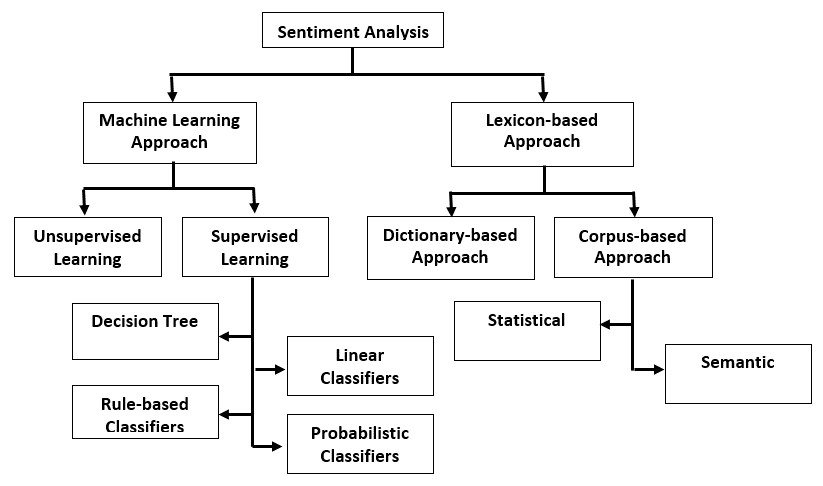
\includegraphics[scale=0.5]{images/learning_approaches_sentiment_analysis}
      \caption[Learning approaches for sentiment analysis]{Learning approaches for sentiment analysis \autocite{Halibas2018}\protect\footnotemark}
      \label{fig:learning_approaches_sentiment_analysis}
    \end{figure}
    
    \footnotetext{\url{https://www.researchgate.net/figure/Sentiment-Analysis-Source-4-Fig-1_fig1_324360275}, (11.04.2019, 23:43)}
    
    Machine learning approaches use mathematical models built by an artificial intelligence to solve the task given to them. They are split into unsupervised and supervised learning. In unsupervised learning no label of a class is provided, so there is no possibility to compare the calculated solution with the correct one. In this case a common learning approach is clustering. The input data is segmented into a (fixed) number of groups, where instances within a group should have similarities and thus form a category. In contrast, there are procedures that are to determine an output value for a given input. These are in the area of supervised learning. While regression methods can handle the assignment of continuous values, classification methods can only be applied if there is a limited and fixed number of possible output values, known as classes. \\\\
    We already defined the domain and codomain of a classification function: $\gamma:\mathbb{X}\rightarrow\mathbb{C}$. Irrespective of the choice of classification algorithm, it is recommended to split the evaluation of the procedure into a training set and a test set. Based on the training set, a model can be created that learns the characteristics of a class. Partly the training set is further subdivided, whereby a model is created on the first part of the training set and fine-tuning is performed by the second part of the set (validation set). During the evaluation the correct classes of the test instances are removed. Without prior viewing, now new classes are assigned to these instances by the learned model, which are then compared with the correct classes. If, as in the case described, only one class is assigned to each instance, it is the hard version of classifying. On the contrary, the soft version assigns to an instance a probabilistic value for each class \autocite{Aggarwal2012}. In the following some such classification learning approaches are introduced, which can be used in the area of text mining:
    \begin{itemize}
      \item Decision Trees
      
        Decision trees are designed with the use of a hierarchical division of the underlying data space with the use of different (text) features. From top to bottom, the partitions become more and more homogeneous by selection of one or several appropriate features for the decision which can be determined by measurement like information gain or Gini coefficient. This procedure can be continued until all leaves are partitions containing only one class. To avoid overfitting and reduce complexity, scarcely informative sections of the tree can be cut by pruning. Finally, a test instance is associated to the class of the partition the decision path starting from the root leads to.
      \item Pattern- or Rule-based Classifiers
      
        Rule-based classifiers are similar to decision trees; more precisely, decision trees can be represented as a set of rules. For each rule the left-hand side is a condition on the underlying feature set (usually expressed in Disjunctive Normal Form (DNF)), and the right-hand side is the class label. A rule should have a high support (absolute number of instances affected by the condition) as well as a high confidence (probability for class if condition is given). In text mining, the rule is typically expressed as a conjunction of terms that have to appear in the instance. The absence of terms is rarely used, because such rules are not likely to be very informative for sparse text data. For any test instance the class of the first rule where the condition is fulfilled will be assigned. That is why the last rule should cover all remaining instances and provide a default class.
      \item Probabilistic Classifiers
      
        Probabilistic classifiers like Bayesian classifiers calculate for each class a probability, whereby the class with the highest value is chosen for the test instance. Naïve Bayes classifiers use therefore the product of all conditional probabilities, e.g. term occurrences in different classes of texts. In comparison to other classifiers, Naïve Bayes classifiers are highly scalable because of its linear complexity. Suitable probabilistic classifiers for text mining are the Bernoulli variate model and multinomial distributions.
      \item SVM Classifiers
      
        Support-vector machines (SVM) are a subgroup of linear classifiers. A linear classifier calculates for a binary classification problem a linear predictor $p=\bar{A}\cdot\bar{X}+b$, where $\bar{X}=(x_{1}...x_{n})$ is the feature vector, $\bar{A}=(a_{1}...a_{n})$ is a vector of linear coefficients with the same dimensionality as the feature space. A natural interpretation of the linear predictor in the discrete scenario would be as a separating hyperplane between the different classes. The hyperplane with the maximum distance value to any instance, i.e. the one with the maximum margin of separation, is chosen. The SVM approach is quite robust to high dimensionality and ideally suited for text data because of the sparse high-dimensional nature of text \autocite{Joachims1997}.
      \item Neural Network Classifiers
      
        Simple neural networks are also a form of linear classifiers, since the function computed by a set of neurons is essentially linear. The simplest form of neural network, known as the perceptron (or single layer network) are essentially designed for linear separation, and work well for text. However, by using multiple layers of neurons, it is also possible to generalize the approach for non-linear separation. In such a network, the outputs of the neurons in the earlier layers feed into the neurons in the later layers. The training process of such networks is more complex, as the errors need to be back-propagated over different layers.
      \item Proximity-based Classifiers
      
        Those classifiers use proximity measures for classification. All training instances are placed in a (high-dimensional) space, proximities of two documents can be calculated by Euclidian, Manhattan or other distance measurements. Then, the most common $k$-nearest-neighbor classifier identifies for a given test instance the $k$ training instances with the smallest distance values. The most common (or highest-weighted) class among them becomes the class of the test instance.
    \end{itemize}
    In the simplest version all of the six classifier types are applied to binary classification problems. If there are three or more classes, the classifier possibly has to be extended to handle this multiclass problem, e.g. for SVM Classifiers. Another possibility is to split the multiclass problem into several binary problems as seen in subsection~\ref{subsec:multiclass_classification}. The classification is made by several classifiers that are trained to differentiate either between one class and the rest (one-against-all) or pairwise between each two classes (one-against-one). Further concepts for the customization of classifiers are boosting and bagging, the formation of ensembles or the handling of ordinal classes \autocite{Aggarwal2012}. \\\\
    For sentiment analysis problems, apart from machine learning approaches also lexicon-based approaches are suitable. Lexicon-based approaches mainly rely on a sentiment lexicon, i.e., a collection of known and precompiled sentiment terms, phrases and even idioms, developed for traditional genres of communication. To determine the polarity score of a text, the polarity scores of the terms are combined in a certain way, e.g. by addition. There are two subtypes of lexicon-based approaches. The dictionary-based approach uses a list of terms called dictionary, where the collection and scores are both created manually. Manual creation may be time-consuming, but it is usually possible to create optimally customized dictionaries with good results. The corpus-based approach uses already existent dictionaries of a specific domain, which have been constructed based on a big corpus. There are statistic techniques like latent semantic analysis (LSA) as well as semantic techniques using synonyms, antonyms or other relationships from thesaurus like WordNet \autocite{Kharde2016}.

  \subsection{Validation and Evaluation}
  \label{subsec:validation_and_evaluation}
    The final step deals with the validation and evaluation of the results obtained from the previous analysis step. In subsection~\ref{subsec:definition_of_the_problem_and_goals} some performance measurements already have been presented. In the following only measurements for classification problems are discussed. Before discussing about those measurements, first of all we will specify how to arrange the data meaningfully to be able to perform most of the measurements. \\\\
    We already mentioned that for the evaluation the data should be split into a training and a test set. Formally speaking, a training set $\mathbb{D}$ of labeled documents $\langle d,c\rangle$ is given, where $\langle d,c\rangle\in\mathbb{X}\times\mathbb{C}$. For all unlabeled documents $d$ in the test set, the chosen classification function(s) $\gamma$ has to predict a class $c$ \autocite[Chapter~13.1]{Manning2008}. Generally, the larger the training set the better the classifier, although the returns begin to diminish once a certain volume of training data is exceeded. And the larger the test set, the more accurate the error estimate. There are different approaches to deal with this problem \autocite[Chapter~5]{Witten2005}:
    \begin{itemize}
      \item Holdout Method
      
        The simplest approach is to determine a specific percentage that should be used for training (usually two thirds). The rest of the data is cut and hold out for the final validation of unseen data. Note that here data can either be used for training or for testing.
      \item k-Fold-Cross-Validation
      
        The cross-validation tries to get away from wasting data by using all data both for training and for testing in different iterations. The data is split into $k$ folds (usually 10); $k-1$ of them are used for training and the remaining one for validation. The final measurement is the average of the measurement of all $k$ iterations and should outbid the simple holdout method in the performance value as well as in its accuracy. A non-random decomposition into folds, e.g. by previous sorting of the data records, can falsify the results.
      \item Leave-One-Out-Validation
      
        For even smaller data sets the leave-one-out-validation is a suitable approach. Here only one test instance is validated while the rest is used for training. This results in $n$ possible iterations where $n$ is the size of the data set. Similar approaches for small data sets with even more possible iterations are the leave-k-out-validation ($\binom{n}{k}$ possiblities) and the bootstrap method \autocite[Chapter~4]{Arlot2010}.
    \end{itemize}
    Of course, it could be also possible not to distinguish between training and test data, i.e. the model is built and evaluated based on all data. However, this approach can lead to overfitted and therefore overestimated performance values that generally cannot be sustained in real application cases when predictions have to be made for unseen data. \\\\
    The accuracy has already been presented as a simple yet meaningful measurement value. Before it is calculated, a confusion matrix $M$ is usually created, where a value $M_{ij}$ specifies how many instances of the class $i$ were classified as class $j$. The accuracy is the sum of all values in the main diagonal of the confusion matrix (i.e. $i=j$) divided by the total number of instances. \\\\
Instead of using an absolute accuracy value it can make sense to use a relative one. In classification problems a baseline can be used as a comparison value for the accuracy. \citeauthor{Witten2005} use an expected value calculated by a default classifier as shown on the right side of table~\ref{tab:actual_and_expected_outcomes_of_three_class_classification}. They assume that the comparison classifier predicts each individual class with the same frequency as the original one. This classifier predicts for $60+18+4=82$ instances the correct class (right side), while the original does for $88+40+12=140$ (left side). This results in $140-82=58$ additional correct classifications out of $200-82=118$ and a kappa statistic of $58\div118=49.2\%$. Another meaningful value to compare is the baseline accuracy, which is achieved by a classifier always selecting the most frequently occurring class. In the example above the baseline classifier achieves $100$ correct classification which would decrease the kappa statistic to $40\%$. Obviously, a kappa statistic of $100\%$ would indicate a perfect classifier, a value of $0\%$ no improvement and a negative value even a deterioration.
  
    \begin{table}[H]
      \begin{tabular}{cc|c|c|c|c|l}
        \cline{3-5}
        & & \multicolumn{3}{ c| }{Predicted class} \\ \cline{3-6}
        & & a & b & c & Total \\ \cline{1-6}
        \multicolumn{1}{ |c  }{\multirow{3}{*}{Actual class} } &
        \multicolumn{1}{ |c| }{a} & 88 & 10 & 2 & 100 & \\ \cline{2-6}
        \multicolumn{1}{ |c  }{} &
        \multicolumn{1}{ |c| }{b} & 14 & 40 & 6 & 60 & \\ \cline{2-6}
        \multicolumn{1}{ |c  }{} &
        \multicolumn{1}{ |c| }{c} & 18 & 10 & 12 & 40 & \\ \cline{1-6}
        \multicolumn{1}{  c  }{} &
        \multicolumn{1}{ |c| }{Total} & 120 & 60 & 20 & 200 & \\ \cline{2-6}
      \end{tabular}      
      \begin{tabular}{cc|c|c|c|c|l}
        \cline{3-5}
        & & \multicolumn{3}{ c| }{Predicted class} \\ \cline{3-6}
        & & a & b & c & Total \\ \cline{1-6}
        \multicolumn{1}{ |c  }{\multirow{3}{*}{Actual class} } &
        \multicolumn{1}{ |c| }{a} & 60 & 30 & 10 & 100 & \\ \cline{2-6}
        \multicolumn{1}{ |c  }{} &
        \multicolumn{1}{ |c| }{b} & 36 & 18 & 6 & 60 & \\ \cline{2-6}
        \multicolumn{1}{ |c  }{} &
        \multicolumn{1}{ |c| }{c} & 24 & 12 & 4 & 40 & \\ \cline{1-6}
        \multicolumn{1}{  c  }{} &
        \multicolumn{1}{ |c| }{Total} & 120 & 60 & 20 & 200 & \\ \cline{2-6}
      \end{tabular}      
      \caption[Outcomes of three-class-classification]{Actual (left) and expected (right) outcomes of three-class-classification, cf.\autocite[Chapter~5.7]{Witten2005}}
      \label{tab:actual_and_expected_outcomes_of_three_class_classification}
    \end{table}
      
    In the kappa statistics just presented it is assumed that all false classifications are equally weighted. However, there are also cases where a classifier with negative kappa statistics is preferable to a baseline classifier. Medical classifications of patients into the classes healthy and sick are a prime example of this. A classifier with $98\%$ accuracy caused by $2\%$ of false positives (healthy patients misclassified as sick) is usually preferable to the baseline classifier with $99\%$ accuracy and the only output healthy and therefore $1\%$ of false negatives (sick patients misclassified as healthy). This is because in this case false negatives weigh heavier than false positives. For this reason, in cost-sensitive classification problems the exact cost factors for each cell in the confusion matrix have to be defined before determining a baseline classifier and an appropriate kappa statistic. In ordinal classification problems the baseline classifier with minimal costs might have the average class as the only output instead of the most common class. The influence of costs in cost-sensitive learning have already been discussed in subsection~\ref{subsec:cost_sensitive_learning}. \\\\
    Apart from the accuracy there are further measurement values like recall and precision. Given the confusion matrix $M$, precision and recall are defined as
    \[precision_{i}=\frac{M_{i i}}{\sum_{j}M_{ji}} \quad \textrm{and} \quad recall_{i}=\frac{M_{i i}}{\sum_{j}M_{ij}}\]
    The precision thus describes how high the quota of correctly classified instances is among all instances classified as class $i$, while the recall describes the quota of correctly classified instances among all instances that actually belong to class $i$. In binary classification problems, the formulas are simplified into
    \[precision=\frac{tp}{tp+fp} \quad \textrm{and} \quad recall=\frac{tp}{tp+fn}\]
    where $tp$ is true positives, $fp$ false positives and $fn$ false negatives. Precision and recall generally have a negative correlation and cannot be optimized at the same time. As a compromise the F-measure can be used which forms the harmonic mean of precision and recall:
    \[F=2\cdot\frac{\text{precision}\cdot\text{recall}}{\text{precision}+\text{recall}}\]
    The Receiver Operating Characteristic (ROC) is an alternative to the precision and recall measurement which visualizes the ratio of true and false positives. The confusion matrix provides only one single point for a classifier, which is generally the better the closer it is to the optimal point (0|1) indicating $0\%$ false positives (and therefore $100\%$ true negatives and optimal precision) and $100\%$ true positives (and therefore $0\%$ false negatives and optimal recall). Because false positives and false negatives can be weighted differently, the Euclidian distance has to be adjusted by different weights for the $x$- and $y$-direction. If the output values of a classifier are ranked (e.g. by probability or relevance), a whole ROC curve can be created
    \begin{itemize}[noitemsep]
      \item starting at the point (0|0),
      \item moving $\frac{1}{P}$ units to the top in case of a true positive (where $P$ is the total number of positives),
      \item moving $\frac{1}{N}$ units to the right in case of a false positive (where $N$ is the total number of negatives)
      \item and ending at the point (1|1).
    \end{itemize}
    In this case, the Area Under ROC Curve (AUC) is another possible indicator for a good classification. It also has a nice interpretation as the probability that the classifier ranks a randomly chosen positive instance above a randomly chosen negative one. Although those definitions and interpretations only work for binary classification problems, there are customized variants for multiclass classification, see \autocite{Hand2001}.

  \clearpage
  
  \section{Experimental Setup}
  \label{sec:experimental_setup}
    In this chapter we consider the general problem described in the previous chapter this time in the field of chess annotations. Therefore, in the beginning of this chapter, the basic chess game format PGN and the corresponding annotations NAGs are introduced. Afterwards we will follow the six steps on which the process is based on. In the following all necessary definitions and tools are presented and some statistics of the data are given. The results of the analysis and their evaluation are discussed in section~\ref{sec:evaluation_of_results}.
    
  \subsection{Problem Description}
    Chess games can be recorded in plain-text-files with the aim of reviewing and analyzing the game later on. Especially in professionally chess tournaments it is common to note not only the player data and the moves, but also some additional information about the game dynamics like an interim position or decisive good or bad moves. There are two ways to describe these game dynamics and annotate the chess game; either by comments in any natural language or by standardized codes and symbols like NAGs. Combinations of both variants are also common. \\\\
    For the evaluation of chess games and their machine processing the unified and structured form given by the standardized codes and symbols is preferable to the unstructured form of the comments in natural language. For chess games which only contain annotations in commentary form, it would therefore be helpful to also provide them with standard codes. This results in the problem of converting the comment into an appropriate code. Using the scheme of \citeauthor{Mitchell1997} presented in subsection~\ref{subsec:definition_of_the_problem_and_goals}, we have:
    \begin{itemize}[noitemsep]
      \item Task $T:$ determine the correct standard code for a given chess annotation comment
      \item Performance measure $P:$ percentage of correctly assigned codes in all code assignments (accuracy)
      \item Experience $E:$ database with tuples of comments and correct codes
    \end{itemize}
      
	\begin{figure}[H]
	  \centering
      \lstset{commentstyle=\color{blue},morecomment=[s]{\{}{\}},moredelim=[is][\bfseries]{\\textbf\{}{\}},moredelim=[is][\color{red}]{\\nag\{}{\}}}
	  \begin{lstlisting}	  
[Event "Deutschland "]
[Site "?"]
[Date "1995.??.??"]
[Round "?"]
[White "Lutz, Ch"]
[Black "Kramnik, V."]
[Result "0-1"]
[ECO "B33"]
[PlyCount "70"]
[EventDate "1995.??.??"]

\textbf{1. e4} {B33: Sicilian: Pelikan and Sveshnikov Variations} \textbf{1... c5 2. Nf3 Nc6 3.
d4 cxd4 4. Nxd4 Nf6 5. Nc3 e5 6. Ndb5 d6 7. Bg5 a6 8. Na3 b5 9. Nd5 Be7 10.
Bxf6 Bxf6 11. c3 O-O 12. Nc2 Bg5 13. a4 bxa4 14. Rxa4 a5 15. Bc4 Rb8 16. b3 Kh8
17. O-O g6 18. Qe2 Bd7 19. Rfa1 19... Bh6} {last book move} \textbf{20. g3} {
Consolidates f4} (20. Nde3 20... Be6 \nag{$14}) \textbf{20... f5} \nag{$11} \textbf{21. exf5 gxf5 22. b4
22... e4} {Black wins space.} \textbf{23. bxa5 Ne5 24. Rb4 Rxb4 25. cxb4 f4 26. Nd4 e3
27. fxe3} (27. Nxf4 \nag{$2} {doesn't work because of} 27... exf2+ 28. Qxf2 28... Bxf4
\nag{$19}) \textbf{27... f3} {He broke from his leash} (27... fxg3 28. hxg3 Qg5 29. Kh2 Nxc4
30. Nf4 \nag{$19}) \textbf{28. Qa2 f2+ 29. Kg2 Qe8 30. Be2 30... Ng4} {
The pressure on the isolated pawn grows} \textbf{31. Bf3} \nag{$4} (31. Qd2 Qh5 32. Bxg4 Qxg4
33. Nf4 Bxf4 34. exf4 Qh3+ 35. Kxf2 Qxh2+ 36. Ke1 Qxg3+ 37. Kd1 Qg1+ 38. Ke2
Bg4+ 39. Kd3 Qxa1 40. f5 \nag{$19}) \textbf{31... Nxe3+} \nag{$19} \textbf{32. Nxe3 Qxe3 33. Qxf2} \nag{$4} {
sad, but how else could White save the game?.} (33. Rd1 Bg7 34. Qb3 Bxd4 35.
Qxe3 Bxe3 36. Be2 \nag{$19}) \textbf{33... Bh3+} \nag{$1} {the final blow} \textbf{34. Kg1} {
Black now must not overlook the idea Re1} (34. Kxh3 {A deflection} 34... Qxf2)
\textbf{34... Qc3 35. Re1 Bd2} (35... Bd2 36. Ne2 36... Qxf3 \nag{$19} (36... Bxe1 \nag{$6} {
is clearly weaker} 37. Nxc3 Bxf2+ 38. Kxf2 \nag{$19}) (36... Rxf3 \nag{$2} 37. Nxc3 Rxf2
38. Kxf2 Bxc3 39. Re7 \nag{$18})) \textbf{0-1}
	  \end{lstlisting}	  

      \caption{Sample PGN game}
      \begin{tabular}{r@{: }l r@{: }l}
        blue & comments & red & NAGs
      \end{tabular}
      \label{fig:sample_pgn_game}
	\end{figure}
	
    Before further specifying the input and output of the task $T$ in subsection~\ref{subsec:problem_specification}, we will first take a closer look at the structure of the chess data. The data sets used for the experience $E$ will be presented in subsection~\ref{subsec:data_set_extraction} and the performance measure $P$ will be adapted to the problem in subsection~\ref{subsec:cost_sensitive_evaluation_methods}.
    
  \subsubsection{PGN Format}
    PGN is "Portable Game Notation", a standard designed for the representation of chess game data using ASCII text files. PGN is structured for easy reading and writing by human users and for easy parsing and generation by computer programs \autocite[Chapter~1]{Edwards1994}. A sample game in PGN notation is shown in figure~\ref{fig:sample_pgn_game}. \\\\
    A PGN game contains first a list of tuples with general information of the game (“tag pairs”). Seven of those tags are mandatory (Seven Tag Roster: Event, Site, Date, Round, White, Black, Result), the other tags are optional. Afterwards the “movetext” section starts. The chess moves themselves are represented using SAN (Standard Algebraic Notation). A move pair (one move of white and one of black) starts with the move pair number followed by a dot and a blank, then the move of white, another blank and the move of black, e.g. 
    \begin{quotation}
      7. Bg5 a6.
    \end{quotation}    
    Each move contains the piece by a single upper-case letter except of the pawn (see table~\ref{tab:basic_chess_notations}) followed by the square the piece is moved to (see figure~\ref{fig:square_names}). Hence, the example describes the seventh move of both players in the game; white moves his dark-squared bishop to the square g5 and black moves his a-file-pawn to a6. If a piece of the opponent is placed on the destination square, this piece is captured and in the move an "x" is inserted immediately before the destination square. In this case, if the capturing piece is a pawn, the lower-case letter of the previous file of the pawn is used at the beginning of the move, e.g. "exd5". Whenever a move pair is interrupted by a comment, the move of black is prefaced by the move pair number, an ellipsis and a blank: 
    \begin{quotation}
      Nxf4 \$2 \{doesn't work because of\} 27... exf2+
    \end{quotation}
    Additionally, there are some further moves with a special notation (see table~\ref{tab:basic_chess_notations}). In cases of disambiguation of pieces, an additional letter for the file or a number for the rank is used. In summary, a move can contain between two and seven signs in SAN \autocite[Chapter~8]{Edwards1994}.
	
    \begin{figure}[H]
      \begin{floatrow}
      \capbtabbox[10.4cm]{%
        \begin{tabular}{| l | l |}
    	\hline
    	Symbol & Meaning \\ \hline
    	  K & King \\ \hline
    	  Q & Queen \\ \hline
    	  R & Rook \\ \hline
    	  B & Bishop \\ \hline
    	  N & Knight \\ \hline
    	  \textit{blank} & Pawn \\ \hline
        \end{tabular}
        \begin{tabular}{| l | l | l |}
    	  \hline
    	  Symbol & Meaning & Example \\ \hline
    	  x & Capture & Rxa1 \\ \hline
    	  + & Check & Nf6+ \\ \hline
    	  \# & Checkmate & Bb7\# \\ \hline
    	  0-0 & Castling kingside & \\ \hline
    	  0-0-0 & Castling queenside & \\ \hline
    	  = & Promotion & fxg1=Q+ \\ \hline
        \end{tabular}
      }{%
        \caption{Basic chess notations}
        \label{tab:basic_chess_notations}
      }
      \ffigbox[6.6cm]{%
	    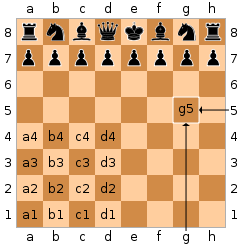
\includegraphics[scale=0.5]{images/algebraic_notation}
      }{%
	    \caption[Square names in algebraic notation]{Square names in algebraic notation\protect\footnotemark}
        \label{fig:square_names}
      }
      \end{floatrow}
    \end{figure}
    
  	\footnotetext{\url{https://en.wikipedia.org/wiki/Algebraic_notation_(chess)#/media/File:SCD_algebraic_notation.svg}, (18.03.2019, 20:56)}
  	
	Parts of the moves are annotated using comments in braces. A comment can contain information about the opening of the game, about a single move or about the current position. In the last two cases the comment is often prefaced by one or several NAGs (see subsection~ref{subsec:nags}) or the corresponding chess symbol. Since there is no restriction on the exact position of a comment, comments may refer to the move before or after itself. A comment can also connect two or more moves with each other. On the contrary, a comment can be interrupted by a move such that it is split into two parts, which may only make sense when seen together. All in all, there are four possibilities of comment-move combinations shown in the examples of table~\ref{tab:comment_move_combinations}.
	
	\begin{table}[H]
      \centering
      \begin{tabular}{| l | l |}
    	\hline
    	Combination & Example \\ \hline
    	Move, Comment & e4 \{Black wins space.\} \\ \hline
    	Comment, Move & \{Weaker is\} 39. Bxe6 \\ \hline
    	Move, Comment, Move & Nxf4 \$2 \{doesn't work because of\} 27... exf2+ \\ \hline
    	Comment, Move, Comment & \{Because of the blunder\} 24. Txf8 \{Black wins immediately\} \\ \hline
      \end{tabular}      
      \caption{Comment-move combinations}
      \label{tab:comment_move_combinations}
    \end{table}
    
    Besides, by convention there should not be nested braces, however, sometimes nested braces are used to comment different move variants separately.	Those variants need not be part of a comment and are written down in parenthesis. The enumeration of the moves proceeds within a variant and is set back before a new variant starts or the game itself continues. 
   
  \subsubsection{NAGs}
  \label{subsec:nags}
    Numeric Annotation Glyphs (NAGs) are used to annotate chess games with assessments of moves or positions in a standard way. They are standard annotation symbols in PGN files, but can as well be used in other chess formats. A NAG is composed of a “\$” followed by one or more digits. There are 140 standard NAGs in total:
    \begin{itemize}[noitemsep]
      \item NAG zero is used as a placeholder
      \item NAGs with values from 1 to 9 annotate the move just played.
      \item NAGs with values from 10 to 135 annotate the current position.
      \item NAGs with values from 136 to 139 describe time pressure.
    \end{itemize}
    The NAGs with values from 140 to 255 are partially defined and used unofficially. The most common NAGs are listed in table~\ref{tab:meaning_of_nags} (see \autocite[Section~10]{Edwards1994}).
	
	\begin{table}[H]
      \subfloat[move-annotating NAGs]{
      \begin{tabular}{| c | c | l |}
    	\hline
    	NAG & Symbol & Meaning \\ \hline
    	\$1 & ! & good move \\ \hline
    	\$2 & ? & poor move \\ \hline
    	\$3 & !! & very good move \\ \hline
    	\$4 & ?? & very poor move \\ \hline
    	\$5 & !? & speculative move \\ \hline
    	\$6 & ?! & questionable move \\ \hline
      \end{tabular}
      }
      \quad
      \subfloat[position-annotating NAGs]{
      \begin{tabular}{| c | c | l |}
    	\hline
    	NAG & Symbol & Meaning \\ \hline
    	\$10 & $=$ & drawish position \\ \hline
    	\$11 &  & equal chances, quiet position \\ \hline
    	\$12 &  & equal chances, active position \\ \hline
    	\$13 & $\infty$ & unclear position \\ \hline
    	\$14 & $+=$ & White has a slight advantage \\ \hline
    	\$15 & $=+$ & Black has a slight advantage \\ \hline
    	\$16 & $\pm$ & White has a moderate advantage \\ \hline
    	\$17 & $\mp$ & Black has a moderate advantage \\ \hline
    	\$18 & $+-$ & White has a decisive advantage \\ \hline
    	\$19 & $-+$ & Black has a decisive advantage \\ \hline
      \end{tabular}
      }
      \caption{Meaning of NAGs}
      \label{tab:meaning_of_nags}
	\end{table}
	
	As shown in table~\ref{tab:meaning_of_nags}, the most common NAGs have a corresponding symbol, which has been used traditionally. Those symbols are composed of the signs “!”, “?”, “+”, “-“, “=” and special signs. It should be emphasized that the subjective symbols do not mix up with the objective move symbols for check and promotion because they are used in different combinations.

  \subsubsection{Problem Specification}
  \label{subsec:problem_specification}
    Now the structure of PGN chess files and the corresponding NAGs being clarified, we can identify use cases in which a sentiment analysis of chess annotations might be useful. In PGN files, comments are often assigned to the NAG that precedes this comment. If no NAG is given - which is the case for more than half of all comments (see table~\ref{tab:flie_statistics}) - we could assign the correct NAG automatically if we would have a reliable learned model. Thus, we will collect the data of already correctly mapped comments and NAGs and recognize contained patterns therein. Concretely, the following problems will be discussed:
    \begin{itemize}
      \item Classification into move and position annotations

      As already seen in table~\ref{tab:meaning_of_nags}, the NAGs are subdivided into NAGs annotating moves and NAGs annotating positions (those describing time pressure are rarely used and therefore negligible). Both annotation types are used at the same place in the PGN file, in particular directly after a move. Therefore, we need to recognize and learn other patterns in order to distinguish these two types of annotations. For this learning problem, the input space $\mathbb{X}$ and output space $\mathbb{C}$ are defined as follows:
      \begin{quotation}
        $\mathbb{X}:=$ set of chess comments without annotation \quad $\mathbb{C}:=\{1,2\}$
      \end{quotation}
      The output class $1$ is used for move annotations and the class $2$ for position annotations. 
      \item Classification of move annotations

      Among the move-annotating NAGs there are basically two groups of annotations; positive and negative ones. It should be noted that positivity and negativity does not refer generally to white or black, but from the viewpoint of the player with the move directly before the NAG. We can formulate the classification problem on the same input space in two degrees of difficulty:
      \begin{quotation}
        $\mathbb{X}:=$ set of move comments without annotation \quad $\mathbb{C}_{1}:=\{1,2\} \quad \mathbb{C}_{2}:=\{1,2,3,4,5,6\}$
      \end{quotation}
      In the first output set, the class $1$ is assigned to all positive move annotations (i.e. \$1, \$3, \$5) and the class $2$ to the negative ones (i.e. \$2, \$4, \$6). In the second output set, each of the six NAGs gets an own class ranked by their “positiveness”. This converts the binary classification problem to an ordinal classification problem with the following mapping of NAGs to classes (1 = most positive, 6 = most negative):
      \begin{quotation}
        $1: \$3$ \quad $2: \$1$ \quad $3: \$5$ \quad $4: \$6$ \quad $5: \$2$ \quad $6: \$4$
      \end{quotation}
      \item Classification of position annotations

      With the position-annotated NAGs we have a similar situation, but with the decisive difference that a neutral class also exists. So even the simpler classification problem already contains three classes:
      \begin{quotation}
        $\mathbb{X}:=$ set of position comments without annotation \quad $\mathbb{C}_{1}:=\{1,2,3\} \quad \mathbb{C}_{2}:=\{1,2,3,4,5,6,7\}$
      \end{quotation}
      In the first output set, the class $1$ is assigned to all position annotations with an advantage of white (i.e. \$14, \$16, \$18), the class $2$ to the balanced position annotations (i.e. \$10, \$11, \$12, \$13) and the class $3$ to the annotations with an advantage of black (i.e. \$15, \$17, \$19). In the second output set, classes $1$ and $3$ are each divided into three subclasses, which makes a total of seven ordered classes (1 = best for white, 7 = best for black):
      \begin{quotation}
        $1: \$18$ \quad $2: \$16$ \quad $3: \$14$ \quad $4: \$10,\$11,\$12,\$13$ \quad $5: \$15$ \quad $6: \$17$ \quad $7: \$19$
      \end{quotation}
    \end{itemize}
    Note that in all cases only one of the output values can be assigned, i.e. we only face single-label problems.
  
  \subsection{Data Set Extraction}
  \label{subsec:data_set_extraction}
  
	\begin{table}[H]
      \subfloat[move-annotating NAGs]{
      \begin{tabular}{| c | c | l |}
    	\hline
    	NAG & Symbol & Meaning \\ \hline
    	\$1 & ! & good move \\ \hline
    	\$2 & ? & poor move \\ \hline
    	\$3 & !! & very good move \\ \hline
    	\$4 & ?? & very poor move \\ \hline
    	\$5 & !? & speculative move \\ \hline
    	\$6 & ?! & questionable move \\ \hline
      \end{tabular}
      }
      \quad
      \subfloat[position-annotating NAGs]{
      \begin{tabular}{| c | c | l |}
    	\hline
    	NAG & Symbol & Meaning \\ \hline
    	\$10 & $=$ & drawish position \\ \hline
    	\$11 &  & equal chances, quiet position \\ \hline
    	\$12 &  & equal chances, active position \\ \hline
    	\$13 & $\infty$ & unclear position \\ \hline
    	\$14 & $+=$ & White has a slight advantage \\ \hline
    	\$15 & $=+$ & Black has a slight advantage \\ \hline
    	\$16 & $\pm$ & White has a moderate advantage \\ \hline
    	\$17 & $\mp$ & Black has a moderate advantage \\ \hline
    	\$18 & $+-$ & White has a decisive advantage \\ \hline
    	\$19 & $-+$ & Black has a decisive advantage \\ \hline
      \end{tabular}
      }
      \caption{Meaning of NAGs}
      \label{tab:file_statistics}
	\end{table}
	
  \subsection{NLTK Processing}
    
   
  \subsection{Attribute Selection}

    
    \newsavebox{\complete}
      \begin{lrbox}{\complete}
        \lstset{keywordstyle=\color{blue},morekeywords={@RELATION,@ATTRIBUTE,@DATA,NUMERIC,REAL}}
        \begin{lstlisting}
@RELATION comment
@ATTRIBUTE COUNT(brilliant) NUMERIC
@ATTRIBUTE TFIDF(mistake) REAL
@ATTRIBUTE CLASS {good,bad}
@DATA
1, 0.0, good
0, 0.06, bad	  
        \end{lstlisting}
      \end{lrbox}
    \newsavebox{\sparse}
      \begin{lrbox}{\sparse}
        \lstset{keywordstyle=\color{blue},morekeywords={@RELATION,@ATTRIBUTE,@DATA,NUMERIC,REAL}}
        \begin{lstlisting}
@RELATION comment
@ATTRIBUTE COUNT(brilliant) NUMERIC
@ATTRIBUTE TFIDF(mistake) REAL
@ATTRIBUTE CLASS {good,bad}
@DATA
{1 2, 3 good}
{2 0.06, 3 bad}	  
        \end{lstlisting}
      \end{lrbox}    
    
    \begin{figure}[H]
	  \centering      
	  \subfloat[complete]{\usebox{\complete}}
	  \quad
	  \subfloat[sparse]{\usebox{\sparse}}
      \caption{Sample arff files}
      \label{fig:sample_arff_files}
	\end{figure}
    
    
  \subsection{Classification Algorithms}
  
    
  \subsection{Cost-sensitive Evaluation Methods}    
  \label{subsec:cost_sensitive_evaluation_methods}

  \clearpage  
  
  \section{Evaluation of Results}
  \label{sec:evaluation_of_results}
    tables with number of attributes, tables with accuracies, comparison of confusion matrix\\
    each for simple approach, tf-idf, word embedding
  \clearpage  
  
  \section{Conclusion}

  \subsection{Summary}

  \subsection{Outlook}
  \clearpage
  
  \paragraph{References}
  \printbibliography
  \clearpage
  
\end{document}
